\documentclass[10pt]{article}
\usepackage{ucs}
\usepackage[a4paper, total={6in, 10in}]{geometry}
\usepackage[utf8x]{inputenc}
\usepackage{graphicx}
\title{Essential Skills: Assignment Operating systems}
\date{30 September 2016}
\author{Ali Abdulmadzhidov}

\begin{document}
\renewcommand*\rmdefault{cmss}
\maketitle
\section{Basic}
\subsection{Find a way to get the name of the host?}
\begin{verbatim}
> hostname
SNE09
\end{verbatim}
\subsection{Find a way to change the time zone manually?}
\begin{verbatim}
> sudo timedatectl set-timezone Europe/Moscow
...
> sudo ln -s /usr/share/zoneinfo/Europe/Moscow /etc/localtime
\end{verbatim}

\subsection{Specify hostnames for an IP address once on the local machine, and then have multiple applications connect to  external resources via their hostnames?}
\begin{verbatim}
> sudo nano /etc/hosts
...
188.130.155.45 mail
...
> ping mail
ping mail
PING mail (188.130.155.45) 56(84) bytes of data.
64 bytes from mail (188.130.155.45): icmp_seq=1 ttl=64 time=0.313 ms
64 bytes from mail (188.130.155.45): icmp_seq=2 ttl=64 time=0.304 ms
^C
--- mail ping statistics ---
2 packets transmitted, 2 received, 0% packet loss, time 1002ms
rtt min/avg/max/mdev = 0.304/0.308/0.313/0.018 ms
> dig ya.ru @mail

; <<>> DiG 9.10.3-P4-Ubuntu <<>> ya.ru @mail
;; global options: +cmd
;; Got answer:
;; ->>HEADER<<- opcode: QUERY, status: NOERROR, id: 22709
;; flags: qr rd ra; QUERY: 1, ANSWER: 3, AUTHORITY: 13, ADDITIONAL: 4

;; OPT PSEUDOSECTION:
; EDNS: version: 0, flags:; udp: 4096
;; QUESTION SECTION:
;ya.ru.             IN  A

;; ANSWER SECTION:
ya.ru.          3423    IN  A   93.158.134.3
ya.ru.          3423    IN  A   213.180.193.3
ya.ru.          3423    IN  A   213.180.204.3
... 
\end{verbatim}


\section{Network}
\subsection{Testing connection}
\begin{verbatim}
> ping 8.8.8.8
PING 8.8.8.8 (8.8.8.8) 56(84) bytes of data.
64 bytes from 8.8.8.8: icmp_seq=1 ttl=55 time=21.3 ms
64 bytes from 8.8.8.8: icmp_seq=2 ttl=55 time=21.2 ms
64 bytes from 8.8.8.8: icmp_seq=3 ttl=55 time=21.2 ms
64 bytes from 8.8.8.8: icmp_seq=4 ttl=55 time=21.2 ms
^C
--- 8.8.8.8 ping statistics ---
4 packets transmitted, 4 received, 0% packet loss, time 3000ms
rtt min/avg/max/mdev = 21.244/21.276/21.349/0.043 ms
\end{verbatim}
\subsection{Provide a report on the path that the packets take to get from the local machine to the remote machine?}
\begin{verbatim}
> traceroute 8.8.8.8
traceroute to 8.8.8.8 (8.8.8.8), 64 hops max, 52 byte packets
 1  192.168.1.1 (192.168.1.1)  3.317 ms  1.277 ms  1.136 ms
 2  10.244.1.1 (10.244.1.1)  1.744 ms  1.631 ms  3.408 ms
 3  10.250.0.1 (10.250.0.1)  1.938 ms  2.014 ms  3.042 ms
 4  37.29.99.73 (37.29.99.73)  4.831 ms  7.358 ms  4.725 ms
 5  192.168.129.1 (192.168.129.1)  14.059 ms  12.849 ms  12.437 ms
 6  10.8.191.26 (10.8.191.26)  11.131 ms  18.223 ms  10.670 ms
 7  10.222.63.226 (10.222.63.226)  23.216 ms  21.979 ms
    10.222.63.224 (10.222.63.224)  26.729 ms
 8  10.222.177.161 (10.222.177.161)  22.239 ms  22.388 ms
    10.222.177.165 (10.222.177.165)  22.056 ms
 9  83.169.204.38 (83.169.204.38)  21.719 ms
    83.169.204.26 (83.169.204.26)  21.497 ms
    83.169.204.34 (83.169.204.34)  54.412 ms
10  37.29.3.250 (37.29.3.250)  25.411 ms
    72.14.222.181 (72.14.222.181)  23.274 ms
    37.29.3.250 (37.29.3.250)  23.254 ms
11  72.14.235.237 (72.14.235.237)  23.316 ms
    72.14.252.62 (72.14.252.62)  23.676 ms
    72.14.235.237 (72.14.235.237)  23.493 ms
12  google-public-dns-a.google.com (8.8.8.8)  40.412 ms  37.951 ms  26.289 ms
\end{verbatim}
\subsection{Speedtest}
We can use python script that uses speedtest.net service
\begin{verbatim}
> wget -O speedtest-cli https://raw.github.com/sivel/speedtest-cli/master/speedtest_cli.py
--2016-09-30 22:50:32--  https://raw.github.com/sivel/speedtest-cli/master/speedtest_cli.py
Resolving raw.github.com... 151.101.84.133
Connecting to raw.github.com|151.101.84.133|:443... connected.
HTTP request sent, awaiting response... 301 Moved Permanently
Location: https://raw.githubusercontent.com/sivel/speedtest-cli/master/speedtest_cli.py [following]
--2016-09-30 22:50:33--  https://raw.githubusercontent.com/sivel/speedtest-cli/master/speedtest_cli.py
Resolving raw.githubusercontent.com... 151.101.84.133
Connecting to raw.githubusercontent.com|151.101.84.133|:443... connected.
HTTP request sent, awaiting response... 200 OK
Length: 24994 (24K) [text/plain]
Saving to: 'speedtest-cli'

speedtest-cli                                   100%[========================================================================================================>]  24.41K  --.-KB/s   in 0.07s

2016-09-30 22:50:34 (362 KB/s) - 'speedtest-cli' saved [24994/24994]

> python speedtest-cli
Retrieving speedtest.net configuration...
Retrieving speedtest.net server list...
Testing from IPADDR.ru (188.130.155.154)...
Selecting best server based on latency...
Hosted by Dataline Ltd (Moscow) [1.61 km]: 28.0 ms
Testing download speed........................................
Download: 25.04 Mbit/s
Testing upload speed..................................................
Upload: 8.72 Mbit/s
\end{verbatim}

Also we can watch network bandwidth with tcptrack or slurm \\ \\

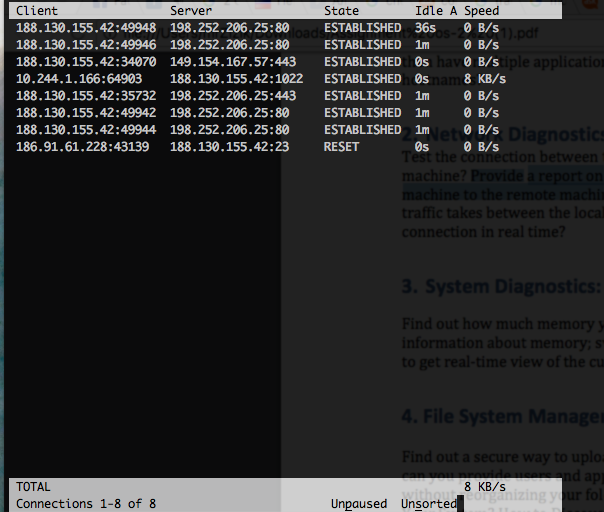
\includegraphics[width=\textwidth]{tcptrack} \\ \\
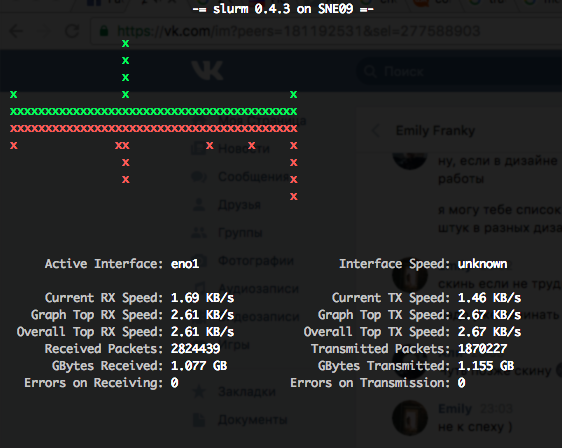
\includegraphics[width=\textwidth]{slurm} 

\section{System diagnostic}
All staff can be done with top or htop. Also we can watch who is working on our system and what they are doing with who or w. \\ \\
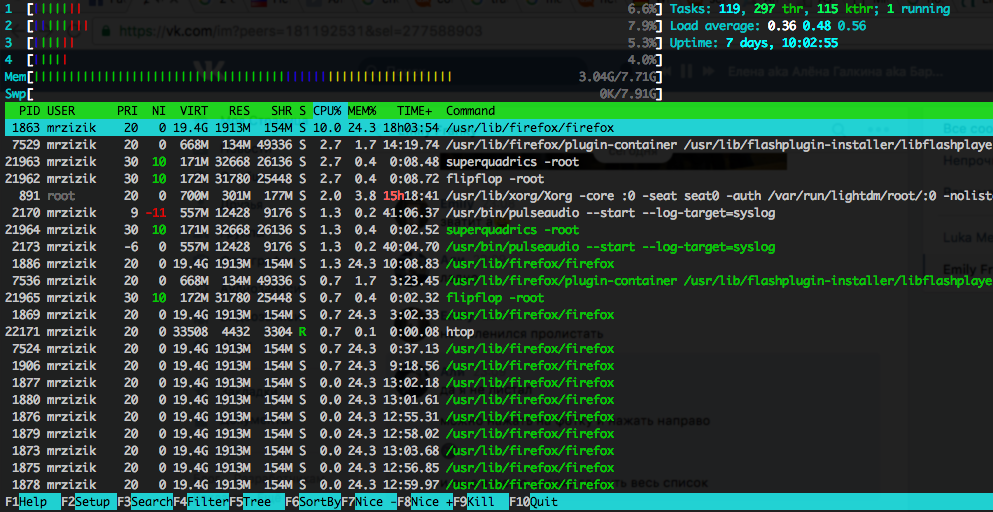
\includegraphics[width=\textwidth, scale=0.5]{htop}\\ \\
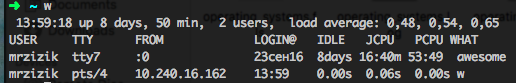
\includegraphics[width=\textwidth, scale=0.5]{w}


\section{File system management}
\subsection{Downloading and uploading files to remote}
\begin{verbatim}
> scp -P 1022 push.sh mrzizik@188.130.155.42:~
mrzizik@188.130.155.42's password:
push.sh                                               100%  129     0.1KB/s   00:00
\end{verbatim}
\begin{verbatim}
> scp -P 1022 mrzizik@188.130.155.42:/home/mrzizik/arch.tar.gz ~/
mrzizik@188.130.155.42's password: 
arch.tar.gz                                           100%  3431KB     3.4MB/s   00:01
\end{verbatim}
\subsection{How can you provide users and applications access to specific files and directories without reorganizing your folders?}
\begin{verbatim}
> chown user:group ~/folder
> chmod 755 ~/folder
\end{verbatim}

\subsection{Strace show specific system calls}
\begin{verbatim}
> strace -e close ls
close(3)                                = 0
close(3)                                = 0
close(3)                                = 0
close(3)                                = 0
close(3)                                = 0
close(3)                                = 0
close(3)                                = 0
close(3)                                = 0
close(3)                                = 0
close(3)                                = 0
...
close(1)                                = 0
close(2)                                = 0
\end{verbatim}

\subsection{Strace show multiple system calls}
\begin{verbatim}
> strace -e trace=close,read ls
close(3)                                = 0
read(3, "\177ELF\2\1\1\0\0\0\0\0\0\0\0\0\3\0>\0\1\0\0\0\260Z\0\0\0\0\0\0"..., 832) = 832
close(3)                                = 0
read(3, "\177ELF\2\1\1\3\0\0\0\0\0\0\0\0\3\0>\0\1\0\0\0P\t\2\0\0\0\0\0"..., 832) = 832
close(3)                                = 0
read(3, "\177ELF\2\1\1\0\0\0\0\0\0\0\0\0\3\0>\0\1\0\0\0000\25\0\0\0\0\0\0"..., 832) = 832
close(3)                                = 0
read(3, "\177ELF\2\1\1\0\0\0\0\0\0\0\0\0\3\0>\0\1\0\0\0\240\r\0\0\0\0\0\0"..., 832) = 832
close(3)                                = 0
read(3, "\177ELF\2\1\1\0\0\0\0\0\0\0\0\0\3\0>\0\1\0\0\0\360`\0\0\0\0\0\0"..., 832) = 832
close(3)                                = 0
read(3, "nodev\tsysfs\nnodev\trootfs\nnodev\tr"..., 1024) = 424
read(3, "", 1024)                       = 0
close(3)                                = 0
close(3)                                = 0
close(3)                                = 0
close(3)                                = 0
...
close(1)                                = 0
close(2)                                = 0
+++ exited with 0 +++
\end{verbatim}

\subsection{Strace running process}
\begin{verbatim}
> sudo strace -p 20952
strace: Process 20952 attached
poll([{fd=3, events=POLLIN|POLLERR}], 1, 718) = 0 (Timeout)
sendmsg(3, {msg_name(16)={sa_family=AF_INET, sin_port=htons(0), sin_addr=inet_addr("127.0.0.1")}, msg_iov(1)=[{"\10\0L\260Q\330\0#$\232\357W\0\0\0\0\206\217\0\0\0\0\0\0\20\21\22\23\24\25\26\27"..., 64}], msg_controllen=0, msg_flags=0}, MSG_CONFIRM) = 64
recvmsg(3, {msg_name(16)={sa_family=AF_INET, sin_port=htons(0), sin_addr=inet_addr("127.0.0.1")}, msg_iov(1)=[{"E\0\0T3+\0\0@\1I|\177\0\0\1\177\0\0\1\0\0T\260Q\330\0#$\232\357W"..., 192}], msg_controllen=32, [{cmsg_len=32, cmsg_level=SOL_SOCKET, cmsg_type=0x1d /* SCM_??? */}], msg_flags=0}, 0) = 84
write(1, "64 bytes from 127.0.0.1: icmp_se"..., 58) = 58
recvmsg(3, 0x7ffd65e32300, 0)           = -1 EAGAIN (Resource temporarily unavailable)
sendmsg(3, {msg_name(16)={sa_family=AF_INET, sin_port=htons(0), sin_addr=inet_addr("127.0.0.1")}, msg_iov(1)=[{"\10\0\361\244Q\330\0$%\232\357W\0\0\0\0\340\231\0\0\0\0\0\0\20\21\22\23\24\25\26\27"..., 64}], msg_controllen=0, msg_flags=0}, MSG_CONFIRM) = 64
recvmsg(3, {msg_name(16)={sa_family=AF_INET, sin_port=htons(0), sin_addr=inet_addr("127.0.0.1")}, msg_iov(1)=[{"E\0\0T3\231\0\0@\1I\16\177\0\0\1\177\0\0\1\0\0\371\244Q\330\0$%\232\357W"..., 192}], msg_controllen=32, [{cmsg_len=32, cmsg_level=SOL_SOCKET, cmsg_type=0x1d /* SCM_??? */}], msg_flags=0}, 0) = 84
write(1, "64 bytes from 127.0.0.1: icmp_se"..., 58) = 58
\end{verbatim}

\subsection{Strace show timestamp}
\begin{verbatim}
strace -t -e close,read ls
14:15:12 close(3)                       = 0
14:15:12 read(3, "\177ELF\2\1\1\0\0\0\0\0\0\0\0\0\3\0>\0\1\0\0\0\260Z\0\0\0\0\0\0"..., 832) = 832
14:15:12 close(3)                       = 0
14:15:12 read(3, "\177ELF\2\1\1\3\0\0\0\0\0\0\0\0\3\0>\0\1\0\0\0P\t\2\0\0\0\0\0"..., 832) = 832
14:15:12 close(3)                       = 0
14:15:12 read(3, "\177ELF\2\1\1\0\0\0\0\0\0\0\0\0\3\0>\0\1\0\0\0000\25\0\0\0\0\0\0"..., 832) = 832
14:15:12 close(3)                       = 0
14:15:12 read(3, "\177ELF\2\1\1\0\0\0\0\0\0\0\0\0\3\0>\0\1\0\0\0\240\r\0\0\0\0\0\0"..., 832) = 832
14:15:12 close(3)                       = 0
14:15:12 read(3, "\177ELF\2\1\1\0\0\0\0\0\0\0\0\0\3\0>\0\1\0\0\0\360`\0\0\0\0\0\0"..., 832) = 832
14:15:12 close(3)                       = 0
14:15:12 read(3, "nodev\tsysfs\nnodev\trootfs\nnodev\tr"..., 1024) = 424
14:15:12 read(3, "", 1024)              = 0
14:15:12 close(3)                       = 0
14:15:12 close(3)                       = 0
14:15:12 close(3)                       = 0
14:15:12 close(3)                       = 0
...
14:15:12 close(1)                       = 0
14:15:12 close(2)                       = 0
14:15:12 +++ exited with 0 +++
\end{verbatim}

\subsection{Find what config program loads on startup}
We can see that php tries to load config from /usr/bin and other dirs, but finds php.ini in /etc/php/7.0/cli/php.ini
\begin{verbatim}
> strace -e open php
open("/etc/ld.so.cache", O_RDONLY|O_CLOEXEC) = 3
open("/lib/x86_64-linux-gnu/libresolv.so.2", O_RDONLY|O_CLOEXEC) = 3
open("/lib/x86_64-linux-gnu/libz.so.1", O_RDONLY|O_CLOEXEC) = 3
open("/lib/x86_64-linux-gnu/libpcre.so.3", O_RDONLY|O_CLOEXEC) = 3
open("/lib/x86_64-linux-gnu/libm.so.6", O_RDONLY|O_CLOEXEC) = 3
open("/lib/x86_64-linux-gnu/libdl.so.2", O_RDONLY|O_CLOEXEC) = 3
open("/usr/lib/x86_64-linux-gnu/libxml2.so.2", O_RDONLY|O_CLOEXEC) = 3
open("/lib/x86_64-linux-gnu/libssl.so.1.0.0", O_RDONLY|O_CLOEXEC) = 3
open("/lib/x86_64-linux-gnu/libcrypto.so.1.0.0", O_RDONLY|O_CLOEXEC) = 3
open("/lib/x86_64-linux-gnu/libc.so.6", O_RDONLY|O_CLOEXEC) = 3
open("/lib/x86_64-linux-gnu/libpthread.so.0", O_RDONLY|O_CLOEXEC) = 3
open("/usr/lib/x86_64-linux-gnu/libicuuc.so.55", O_RDONLY|O_CLOEXEC) = 3
open("/lib/x86_64-linux-gnu/liblzma.so.5", O_RDONLY|O_CLOEXEC) = 3
open("/usr/lib/x86_64-linux-gnu/libicudata.so.55", O_RDONLY|O_CLOEXEC) = 3
open("/usr/lib/x86_64-linux-gnu/libstdc++.so.6", O_RDONLY|O_CLOEXEC) = 3
open("/lib/x86_64-linux-gnu/libgcc_s.so.1", O_RDONLY|O_CLOEXEC) = 3
open("/usr/lib/locale/locale-archive", O_RDONLY|O_CLOEXEC) = 3
open("/etc/localtime", O_RDONLY|O_CLOEXEC) = 3
open("/usr/bin/php-cli.ini", O_RDONLY)  = -1 ENOENT (No such file or directory)
open("/etc/php/7.0/cli/php-cli.ini", O_RDONLY) = -1 ENOENT (No such file or directory)
open("/usr/bin/php.ini", O_RDONLY)      = -1 ENOENT (No such file or directory)
open("/etc/php/7.0/cli/php.ini", O_RDONLY) = 3
...
\end{verbatim}

\subsection{Find where program spends most time}
We can see that php tries to load config from /usr/bin and other dirs, but finds php.ini in /etc/php/7.0/cli/php.ini
\begin{verbatim}
> strace sudo apt update
...
% time     seconds  usecs/call     calls    errors syscall
------ ----------- ----------- --------- --------- ----------------
 77.69    0.148592       12383        12           wait4
 18.13    0.034666          60       574           write
  4.18    0.008000         229        35         3 unlink
  0.00    0.000000           0      5412           read
  0.00    0.000000           0       431        42 open
  0.00    0.000000           0       431           close
  0.00    0.000000           0      1767       980 stat
  0.00    0.000000           0       424           fstat
  0.00    0.000000           0         9           lstat
  0.00    0.000000           0       118           lseek
  0.00    0.000000           0       113           mmap
  0.00    0.000000           0        33           mprotect
  0.00    0.000000           0        61           munmap
  0.00    0.000000           0        65           brk
  0.00    0.000000           0         4           rt_sigaction
  0.00    0.000000           0        72           rt_sigprocmask
  0.00    0.000000           0         4           ioctl
  0.00    0.000000           0        19        18 access
  0.00    0.000000           0        19           pipe
  0.00    0.000000           0        64           select
  0.00    0.000000           0        20           mremap
  0.00    0.000000           0         1           getpid
  0.00    0.000000           0         4           socket
  0.00    0.000000           0         4         4 connect
  0.00    0.000000           0        12           clone
  0.00    0.000000           0         1           execve
  0.00    0.000000           0         8           kill
  0.00    0.000000           0       310           fcntl
  0.00    0.000000           0        18           getdents
  0.00    0.000000           0         2           getcwd
  0.00    0.000000           0         4           chdir
  0.00    0.000000           0         7           rename
  0.00    0.000000           0        24           chmod
  0.00    0.000000           0         4           fchmod
  0.00    0.000000           0        24           chown
  0.00    0.000000           0         6           umask
  0.00    0.000000           0        26           getuid
  0.00    0.000000           0        14           geteuid
  0.00    0.000000           0         1           getegid
  0.00    0.000000           0         1           getgroups
  0.00    0.000000           0         2           setgroups
  0.00    0.000000           0         2           setresuid
  0.00    0.000000           0         2           setresgid
  0.00    0.000000           0         1           arch_prctl
------ ----------- ----------- --------- --------- ----------------
100.00    0.191258                 10165      1047 total
...
\end{verbatim}

\subsection{Find why program can't connect to server}
I broke dns on my machine, so we can see that in that part wget tries to resolve ya.ru, but it can't
\begin{verbatim}
> strace -e poll,select,connect,recvfrom,sendto wget ya.ru
--2016-10-01 14:48:12--  http://ya.ru/
Resolving ya.ru (ya.ru)... connect(3, {sa_family=AF_LOCAL, sun_path="/var/run/nscd/socket"}, 110) = -1 ENOENT (No such file or directory)
connect(3, {sa_family=AF_LOCAL, sun_path="/var/run/nscd/socket"}, 110) = -1 ENOENT (No such file or directory)
connect(3, {sa_family=AF_INET, sin_port=htons(53), sin_addr=inet_addr("127.0.0.1")}, 16) = 0
poll([{fd=3, events=POLLOUT}], 1, 0)    = 1 ([{fd=3, revents=POLLOUT}])
poll([{fd=3, events=POLLIN}], 1, 5000)  = 1 ([{fd=3, revents=POLLIN}])
recvfrom(3, "U.\201\5\0\1\0\0\0\0\0\0\2ya\2ru\0\0\1\0\1", 2048, 0, {sa_family=AF_INET, sin_port=htons(53), sin_addr=inet_addr("127.0.0.1")}, [16]) = 23
poll([{fd=3, events=POLLIN}], 1, 4999)  = 1 ([{fd=3, revents=POLLIN}])
recvfrom(3, ".\5\201\5\0\1\0\0\0\0\0\0\2ya\2ru\0\0\34\0\1", 65536, 0, {sa_family=AF_INET, sin_port=htons(53), sin_addr=inet_addr("127.0.0.1")}, [16]) = 23
poll([{fd=3, events=POLLOUT}], 1, 0)    = 1 ([{fd=3, revents=POLLOUT}])
poll([{fd=3, events=POLLIN}], 1, 5000)  = 1 ([{fd=3, revents=POLLIN}])
recvfrom(3, "U.\201\5\0\1\0\0\0\0\0\0\2ya\2ru\0\0\1\0\1", 2048, 0, {sa_family=AF_INET, sin_port=htons(53), sin_addr=inet_addr("127.0.0.1")}, [16]) = 23
poll([{fd=3, events=POLLIN}], 1, 4999)  = 1 ([{fd=3, revents=POLLIN}])
recvfrom(3, ".\5\201\5\0\1\0\0\0\0\0\0\2ya\2ru\0\0\34\0\1", 65536, 0, {sa_family=AF_INET, sin_port=htons(53), sin_addr=inet_addr("127.0.0.1")}, [16]) = 23
connect(3, {sa_family=AF_INET, sin_port=htons(53), sin_addr=inet_addr("127.0.0.1")}, 16) = 0
poll([{fd=3, events=POLLOUT}], 1, 0)    = 1 ([{fd=3, revents=POLLOUT}])
poll([{fd=3, events=POLLIN}], 1, 5000)  = 1 ([{fd=3, revents=POLLIN}])
recvfrom(3, "\343\324\201\5\0\1\0\0\0\0\0\0\2ya\2ru\0\0\1\0\1", 2048, 0, {sa_family=AF_INET, sin_port=htons(53), sin_addr=inet_addr("127.0.0.1")}, [16]) = 23
poll([{fd=3, events=POLLIN}], 1, 4999)  = 1 ([{fd=3, revents=POLLIN}])
recvfrom(3, "h\250\201\5\0\1\0\0\0\0\0\0\2ya\2ru\0\0\34\0\1", 65536, 0, {sa_family=AF_INET, sin_port=htons(53), sin_addr=inet_addr("127.0.0.1")}, [16]) = 23
poll([{fd=3, events=POLLOUT}], 1, 0)    = 1 ([{fd=3, revents=POLLOUT}])
poll([{fd=3, events=POLLIN}], 1, 5000)  = 1 ([{fd=3, revents=POLLIN}])
recvfrom(3, "\343\324\201\5\0\1\0\0\0\0\0\0\2ya\2ru\0\0\1\0\1", 2048, 0, {sa_family=AF_INET, sin_port=htons(53), sin_addr=inet_addr("127.0.0.1")}, [16]) = 23
poll([{fd=3, events=POLLIN}], 1, 4999)  = 1 ([{fd=3, revents=POLLIN}])
recvfrom(3, "h\250\201\5\0\1\0\0\0\0\0\0\2ya\2ru\0\0\34\0\1", 65536, 0, {sa_family=AF_INET, sin_port=htons(53), sin_addr=inet_addr("127.0.0.1")}, [16]) = 23
...
\end{verbatim}

\end{document}